%package list
\documentclass{article}
\usepackage[top=3cm, bottom=3cm, outer=3cm, inner=3cm]{geometry}
\usepackage{graphicx}
\usepackage{url}
\usepackage{multirow}
%\usepackage{cite}
\usepackage{hyperref}
\usepackage{array}
\usepackage{multicol}
\newcolumntype{x}[1]{>{\centering\arraybackslash\hspace{0pt}}p{#1}}
\usepackage{natbib}
\usepackage{pdfpages}
\usepackage{multirow}
\usepackage{float}
\usepackage[normalem]{ulem}
\useunder{\uline}{\ul}{}




%%%%%%%%%%%%%%%%%%%%%%%%%%%%%%%%%%%%%%%%%%%%%%%%%%%%%%%%%%%%%%%%%%%%%%%%%%%%
%%%%%%%%%%%%%%%%%%%%%%%%%%%%%%%%%%%%%%%%%%%%%%%%%%%%%%%%%%%%%%%%%%%%%%%%%%%%
\newcommand{\csemail}{vmachacaa@unsa.edu.pe}
\newcommand{\csdocente}{Vicente Machaca Arceda}
\newcommand{\cscurso}{Algoritmos y Estructura de Datos}
\newcommand{\csuniversidad}{Universidad Nacional de San Agustín}
\newcommand{\csescuela}{Maestría en Ciencia de la Computación}
\newcommand{\cspracnr}{01}
\newcommand{\cstema}{--}
%%%%%%%%%%%%%%%%%%%%%%%%%%%%%%%%%%%%%%%%%%%%%%%%%%%%%%%%%%%%%%%%%%%%%%%%%%%%
%%%%%%%%%%%%%%%%%%%%%%%%%%%%%%%%%%%%%%%%%%%%%%%%%%%%%%%%%%%%%%%%%%%%%%%%%%%%


\usepackage[english,spanish]{babel}
\usepackage[utf8]{inputenc}
\AtBeginDocument{\selectlanguage{spanish}}
\renewcommand{\figurename}{Figura}
\renewcommand{\refname}{Referencias}
\renewcommand{\tablename}{Tabla} %esto no funciona cuando se usa babel
\AtBeginDocument{%
	\renewcommand\tablename{Tabla}
}

\usepackage{fancyhdr}
\pagestyle{fancy}
\fancyhf{}
\setlength{\headheight}{30pt}
\renewcommand{\headrulewidth}{1pt}
\renewcommand{\footrulewidth}{1pt}
\fancyhead[L]{\raisebox{-0.2\height}{
\includegraphics[width=3cm]{Imagen/logo_unsa}}}
\fancyhead[C]{}
\fancyhead[R]{\fontsize{7}{7}\selectfont	\csuniversidad \\ \csescuela \\ \textbf{\cscurso} }
\fancyfoot[L]{MSc. Vicente Machaca}
\fancyfoot[C]{\cscurso}
\fancyfoot[R]{Página \thepage}







\begin{document}
	
	\vspace*{10px}
	
	\begin{center}	
		\fontsize{17}{17} \textbf{ Práctica \cspracnr}
	\end{center}
	%\centerline{\textbf{\underline{\Large Título: Informe de revisión del estado del arte}}}
	%\vspace*{0.5cm}
	

	\begin{table}[h]
		\begin{tabular}{|x{4.7cm}|x{4.8cm}|x{4.8cm}|}
			\hline 
			\textbf{DOCENTE} & \textbf{CARRERA}  & \textbf{CURSO}   \\
			\hline 
			\csdocente & \csescuela & \cscurso    \\
			\hline 
		\end{tabular}
	\end{table}	
	
	
	\begin{table}[h]
		\begin{tabular}{|x{4.7cm}|x{4.8cm}|x{4.8cm}|}
			\hline 
			\textbf{PRÁCTICA} & \textbf{TEMA}  & \textbf{DURACIÓN}   \\
			\hline 
			\cspracnr & Algoritmos de ordenamiento  & 3 horas   \\
			\hline 
		\end{tabular}
	\end{table}
	
	
	\section{Datos de los estudiantes}
	Grupo: N° 8
	\begin{itemize}
		\item Integrantes: 
		\begin{itemize}
			\item Esai Josue Huaman Meza
			\item Alan Jerry Reyes Robles
			\item Jorge Luis Zegarra Guardamino
			\item Nestor Giraldo Calcinas Huaranga
		\end{itemize}		
	\end{itemize}
	
	
	
	
	
	
	\section{Introducción}
	
	Se hara un análisis comparativo 04 algoritmos de ordenamiento, buscando estudiar la complejidad de cada uno de estos y como las diferentes formas de resolver un mismo problema pueden afectar los tiempos de ejecución, esto se hara en 3 lenguales de programacion: C++, Go y Python.
	
	Dado que para hacer un buen análisis se deben correr muchas pruebas, se implementa codigo que me permitieran automatizarlas de forma tal que se pudieran correr de forma continua sin intervención. Se creara un pequeño ambiente controlado por lo que se usara una sola PC para realizar las pruebas donde no estuvieran ejecutandose en paralelo otras tareas, dado que los tiempos de ejecución de cada prueba puede verse afectado al estar compartiendo recursos con otros procesos.

    Se corrieron las pruebas con el mismo archivo de numeros aleatorios a ordenar, en intervalos de 100, luego de 1000 en 1000, luego de 10.000 en 10.000, hasta 50.000 datos, estos resultados se guardaran en archivos CSV para poder visualizar luego con python.
	

	
	\section{Algoritmos de Ordenamiento}\label{sec:ejercicios}
	\begin{enumerate}
		\item \textbf{Algoritmo Counting Sort}
		
			Counting sort es un algoritmo de ordenación que ordena los elementos de una matriz contando el número de apariciones de cada elemento único de la matriz. El recuento se almacena en una matriz auxiliar y la clasificación se realiza asignando el recuento como un índice de la matriz auxiliar.
			
La clasificación de conteo se ejecuta en un conjunto de entrada relativamente más pequeño. Counting sort calcula, para cada elemento en el arreglo - X, el número de elementos que son menores que - X. Luego usa esta información para colocar X directamente en su posición en el arreglo ordenado.

La ordenación por selección toma dos arreglos adicionales.

\begin{itemize}
   \item Uno para el resultado, la matriz ordenada
   \item otro para almacenamiento temporal, donde el tamaño es   igual al número máximo en la matriz de entrada.
 \end{itemize}	
 
 Es interesante notar que este algoritmo no es un tipo de comparación. No verá ninguna comparación en el código. Este algoritmo utiliza valores de elementos para indexar en una matriz.
		
\begin{figure}[H]
\centering
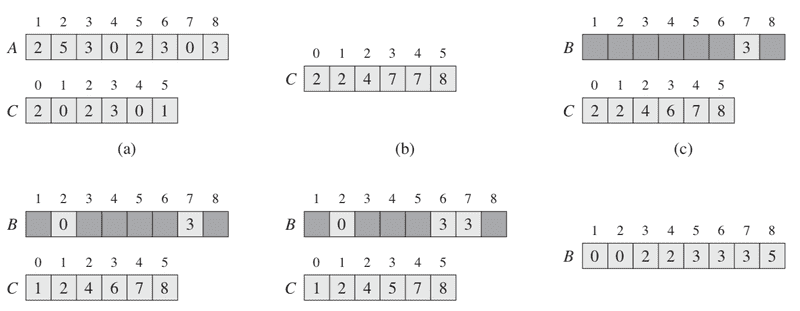
\includegraphics[width=0.7\textwidth]{Imagen/CountS}
\caption{Algoritmo Counting Sort}
\label{fig:CountS}
\end{figure}



\item \textbf{Algoritmo Merge Sort}
        
		 El algoritmo de ordenamiento por mezcla (merge sort) es un algoritmo de ordenamiento externo estable basado en la técnica divide y vencerás.
		 
        La idea de los algoritmos de ordenación por mezcla es dividir la matriz por la mitad una y otra vez hasta que cada pieza tenga solo un elemento de longitud. Luego esos elementos se vuelven a juntar (mezclados) en orden de clasificación.
        
        Conceptualmente, el ordenamiento por mezcla funciona de la siguiente manera: 
        \begin{itemize}
            \item Si la longitud de la lista es 0 o 1, entonces ya está ordenada.
        \end{itemize}
    
        En otro caso: 
        \begin{itemize}
            \item Dividir la lista desordenada en dos sublistas de aproximadamente la mitad del tamaño. 
            \item Ordenar cada sublista recursivamente aplicando el ordenamiento por mezcla. 
            \item Mezclar las dos sublistas en una sola lista ordenada.
        \end{itemize}

        El ordenamiento por mezcla incorpora dos ideas principales para mejorar su tiempo de ejecución:
        \begin{enumerate}
            \item Una lista pequeña necesitará menos pasos para ordenarse que una lista grande.
        \end{enumerate}
        \begin{enumerate}
            \item Se necesitan menos pasos para construir una lista ordenada a partir de dos listas también ordenadas, que a partir de dos listas desordenadas.
        \end{enumerate}
    
        
    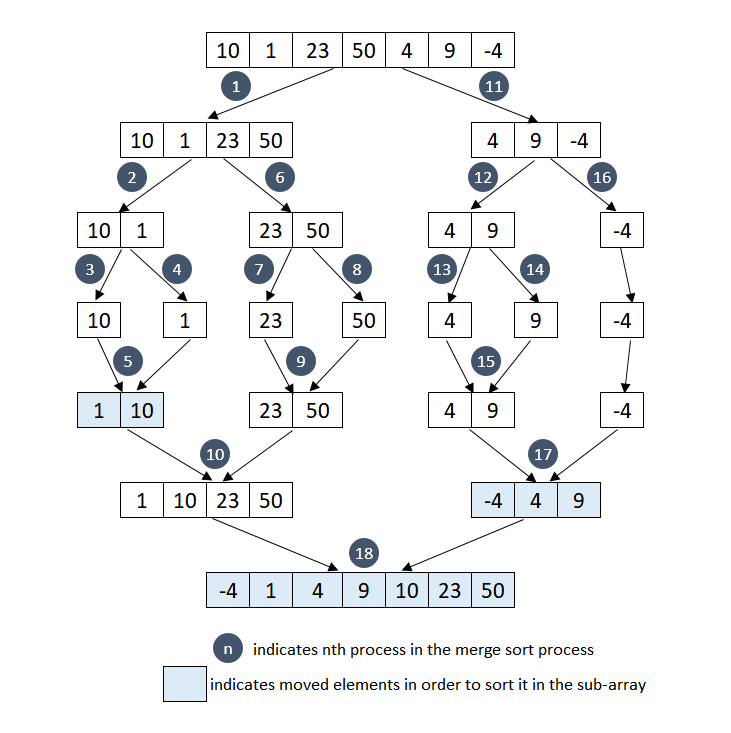
\includegraphics[width=0.8\textwidth]{Imagen/merge-sort}
    
    
            Este tipo de ordenamiento es útil cuando se tiene una estructura ordenada y los nuevos datos a añadir se almacenan en una estructura temporal para después agregarlos a la estructura original de manera que vuelva a quedar ordenada.
        
    
    
        \begin{enumerate}
            \item {Coste Computacional}
                    
                    En todos los casos (el peor, el promedio y el mejor), el algoritmo Merge Sort siempre divide la matriz hasta que todas las submatrices contienen un solo elemento y tarda un tiempo lineal en fusionar esas submatrices. El proceso de división tiene una complejidad de tiempo $\Theta (logN)$ y el proceso de fusión tiene una complejidad de tiempo $\Theta (N)$. Por lo tanto, en todos los casos, la complejidad temporal del algoritmo Merge Sort es $\Theta(NlogN)$.

                    
                    Merge sort es un ordenamiento estable, paraleliza mejor, y es más eficiente manejando medios secuenciales de acceso lento. 
            
        \end{enumerate}

	
\item \textbf{Algoritmo Heap Sort}

        Heapsort. Proviene del inglés y significa ordenamiento por montículos. Es un algoritmo de ordenaciónno recursivo, no estable, con complejidad computacional O (n log n).
		
        Este algoritmo consiste en almacenar todos los elementos del vector a ordenar en un montículo (heap), y luego extraer el nodo que queda como nodo raíz del montículo (cima) en sucesivas iteraciones obteniendo el conjunto ordenado. Basa su funcionamiento en una propiedad de los montículos, por la cual, la cima contiene siempre el menor elemento (o el mayor, según se haya definido el montículo) de todos los almacenados en él.
        
        Conceptualmente, el ordenamiento por montículos funciona de la siguiente manera:
        
        \begin{itemize}
            \item Construir un Heap sobre el arreglo a ordenar (BUILD HEAP), en orden contrario 
            al orden de ordenación. Por ejemplo, para ordenar ascendentemente un arreglo se 
            construye un HEAP sobre él de forma descendiente (el mayor elemento queda en la raíz).

            \item Intercambiar la raíz del Heap, posición 0, con la ultima posición en el Heap.

            \item Disminuir el tamaño del Heap.

            \item Reconstruir el Heap aplicando Heapify en la primera posición.

            \item Repetir los pasos 2, 3 y 4 mientras el tamaño del Heap sea mayor que uno.
            
        \end{itemize}	
		
	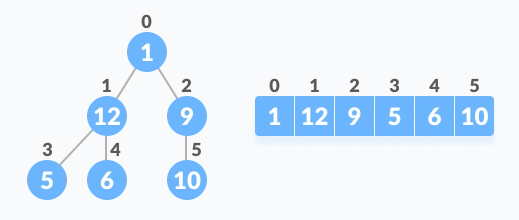
\includegraphics[width=\textwidth]{Imagen/hs1}		
	    \item \textbf{Algoritmo Quicksort}
     
     El algoritmo de Ordenamiento Rápido o también llamado Quick Sort fue creado por el científico Británico en computación Charles Antony Richard Hoare.
     
     Este ordenamiento trabaja de la siguiente manera:
     \begin{itemize}
            \item Se elige un elemento de un conjuntos de elementos al que se llamará pivote.
            \item Se reordenan los elementos a cada lado del pivote, tomando en cuenta que a un lado queden los elementos menores al pivote y al otro lado los elementos mayores al pivote, para aquellos elementos iguales al pivote, se pueden colocar a cualquier lado de este, para este paso, el pivote ocupa el lugar que le corresponde en la lista.
            \item La lista queda separada en dos sublistas, una lista de elementos menores al pivote, y otra lista de elementos mayores al pivote.
            \item Se repite los pasos del punto dos, mientras éstas contengan más de un elemento en cada sublista.
        \end{itemize}
        
    Para este tipo de ordenamiento existen tres casos para poder suponer la eficiencia del algoritmo:
     \begin{itemize}
            \item En el mejor de los casos, el pivote termina en el centro de la lista, diviendo la lista en dos sublistas de igual tamaño. En este caso la complejidad del algoritmo es $\Theta(n.log n)$.
            \item En el peor de los casos, el pivote termina a un extremo de la lista. En este caso la complejidad del algoritmo es $\Theta (n^2)$.
            \item En el caso promedio, el orden es $\Theta (n.log n)$.
    \end{itemize}

\begin{figure}[H]
\centering
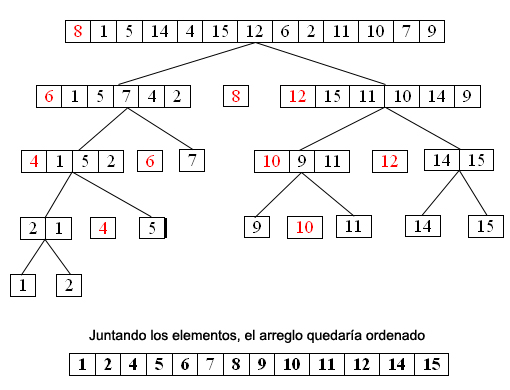
\includegraphics[width=0.7\textwidth]{Imagen/Ejem_QuickSort.jpg}
\caption{Ordenamiento QuickSort}
\label{fig:QuickSort}
\end{figure}

   Para esta Práctica 01, se ha realizado el Ordenamiento Rápido (QuickSort) en 03 tipos de lenguajes de programación (Goland, Python y C++), para identificar el Tiempo de Procesamiento y la Desviación Estandar en cada lenguaje.

   Para medir el tiempo, se da diferentes tamaños de datos que varían de 100,1000, 2000, 3000, 4000, 5000, 6000, 7000, 8000, 9000, 10000, 20000, 30000, 40000 y 50000 datos.

\end{enumerate}


\section{Implementación}

  Se desarrollan los diferentes algoritmos en los 03 tipos de lenguajes antes mencionados, los cuales se pueden encontrar en el siguiente repositorio Github \href{https://github.com/josuemzx/Algoritmos_de_ordenamiento-/blob/main/Practica01_QuickSort.ipynb}{Algoritmos QuickSort}, y se obtiene la siguiente tabla con los siguientes gráficos:


\section{Resultados}


    \begin{enumerate}
        \item Información del Sistema
        
        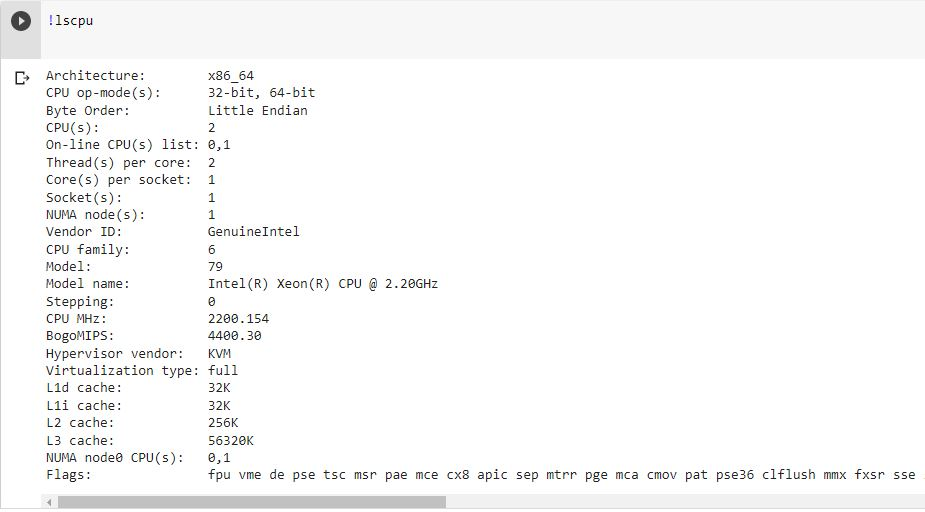
\includegraphics[width=\textwidth]{Imagen/Captura1}
	   
        \item Algoritmo Counting Sort
        
        \begin{tabular}{ |p{0.3cm}||p{0.9cm}|p{1.5cm}|p{1.7cm}|p{1.5cm}|p{1.7cm}|p{1.8cm}|p{1.7cm}|  }
 \hline
 \multicolumn{8}{|c|}{Tabla comparativa con el promedio de tiempo de procesamiento y desviación estandar} \\
 \hline
 N°& Datos &Python Promedio &Python Desviación Estandar &C++ Promedio &C++ Desviación Estandar &GO Promedio &GO Desviación Estandar\\
 \hline
0 &100 &0.008069 &0.000143	&0.000292 &0.000066 &0.000109 &0.000020\\
1 &1000	&0.010068	&0.000754	&0.000274	&0.000003	&0.000103	&0.000018\\
2	&2000	&0.010750	&0.000729	&0.000284	&0.000002	&0.000111	&0.000022\\
3	&3000	&0.011239	&0.000335	&0.000302	&0.000003	&0.000099	&0.000017\\
4	&4000	&0.014080	&0.002667	&0.000314	&0.000002	&0.000103	&0.000022\\
5	&5000	&0.013084	&0.001839	&0.000330	&0.000010	&0.000119	&0.000039\\
6	&6000	&0.012468	&0.000601	&0.000346	&0.000014	&0.000101	&0.000019\\
7	&7000	&0.014128	&0.002605	&0.000356	&0.000006	&0.000108	&0.000023\\
8	&8000	&0.013761	&0.000387	&0.000365	&0.000004	&0.000114	&0.000020\\
9	&9000	&0.013874	&0.000234	&0.000383	&0.000012	&0.000112	&0.000020\\
10	&10000	&0.014682	&0.000361	&0.000394	&0.000007	&0.000112	&0.000022\\
11	&20000	&0.024680	&0.003192	&0.000543	&0.000041	&0.000123	&0.000045\\
12	&30000	&0.029446	&0.001843	&0.000660	&0.000032	&0.000118	&0.000030\\
13	&40000	&0.038761	&0.002477	&0.000796	&0.000040	&0.000102	&0.000019\\
14	&50000	&0.045249	&0.003135	&0.000930	&0.000045	&0.000121	&0.000045\\
\hline
\end{tabular}


\begin{figure}[H]
\centering
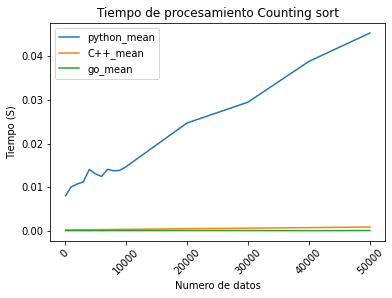
\includegraphics[width=0.8\textwidth]{Imagen/CS1.png}
\label{fig:QuickSort}
\end{figure}

\begin{figure}[H]
\centering
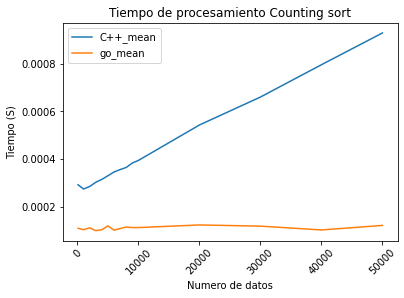
\includegraphics[width=0.8\textwidth]{Imagen/CS2.png}
\label{fig:QuickSort}
\end{figure}
\begin{figure}[H]
\centering
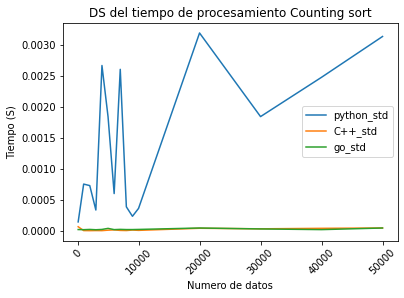
\includegraphics[width=0.8\textwidth]{Imagen/CS3.png}
\label{fig:QuickSort}
\end{figure}

\begin{figure}[H]
\centering
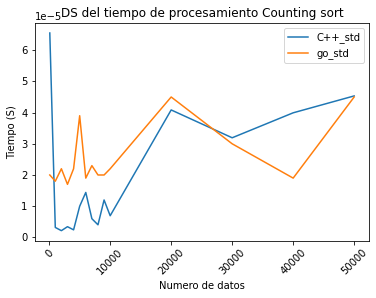
\includegraphics[width=0.8\textwidth]{Imagen/CS4.png}
\label{fig:QuickSort}
\end{figure}


        
        
        \item Algoritmo Merge Sort
        
 \begin{tabular}{ |p{0.3cm}||p{0.9cm}|p{1.5cm}|p{1.7cm}|p{1.5cm}|p{1.7cm}|p{1.8cm}|p{1.7cm}|  }
 \hline
 \multicolumn{8}{|c|}{Tabla comparativa con el promedio de tiempo de procesamiento y desviación estandar} \\
 \hline
 N°& Datos &Python Promedio &Python Desviación Estandar &C++ Promedio &C++ Desviación Estandar &GO Promedio &GO Desviación Estandar\\
 \hline
1	&100	&0.000303	&0.000008	&0.000010	&0.000003	&0.000083	&0.000016\\
2	&1000	&0.004241	&0.000062	&0.000108	&0.000026	&0.000093	&0.000037\\
3	&2000	&0.009230	&0.000146	&0.000228	&0.000054	&0.000087	&0.000033\\
4	&3000	&0.014717	&0.000384	&0.000357	&0.000083	&0.000086	&0.000029\\
5	&4000	&0.020847	&0.001502	&0.000489	&0.000112	&0.000091	&0.000020\\
6	&5000	&0.029228	&0.003743	&0.000622	&0.000143	&0.000093	&0.000019\\
7	&6000	&0.031280	&0.000499	&0.000752	&0.000181	&0.000099	&0.000016\\
8	&7000	&0.037319	&0.001077	&0.000887	&0.000218	&0.000101	&0.000022\\
9	&8000	&0.043424	&0.001824	&0.001037	&0.000279	&0.000113	&0.000028\\
10	&9000	&0.050214	&0.001805	&0.001167	&0.000302	&0.000111	&0.000024\\
11	&10000	&0.059206	&0.005889	&0.001315	&0.000324	&0.000112	&0.000031\\
12	&20000	&0.121145	&0.002702	&0.002768	&0.000665	&0.000114	&0.000022\\
13	&30000	&0.195814	&0.006638	&0.004234	&0.001095	&0.000115	&0.000027\\
14	&40000	&0.271920	&0.011808	&0.005800	&0.001428	&0.000113	&0.000023\\
15	&50000	&0.339185	&0.008188	&0.007354	&0.001819	&0.000125	&0.00002\\

\hline
\end{tabular}

\begin{figure}[H]
\centering
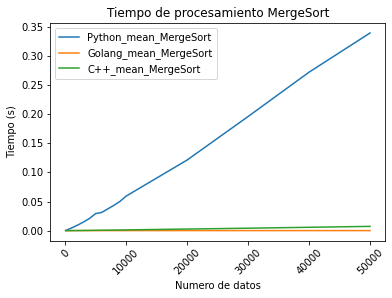
\includegraphics[width=0.8\textwidth]{Imagen/merge_prom.png}
\caption{Tiempo de Procesamiento MergeSort}
\label{fig:QuickSort}
\end{figure}

\begin{figure}[H]
\centering
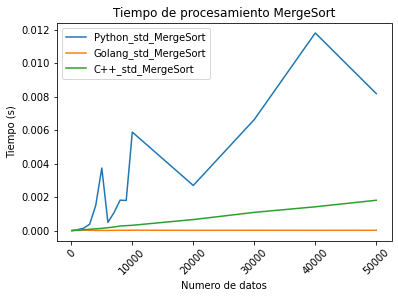
\includegraphics[width=0.8\textwidth]{Imagen/merge_sd.png}
\caption{Desviación Estandar MergeSort}
\label{fig:QuickSort}
\end{figure}
        
        \item Algoritmo Heap Sort
	
\begin{tabular}{ |p{0.3cm}||p{0.9cm}|p{1.5cm}|p{1.7cm}|p{1.5cm}|p{1.7cm}|p{1.8cm}|p{1.7cm}|  }
 \hline
 \multicolumn{8}{|c|}{Tabla comparativa con el promedio de tiempo de procesamiento y desviación estandar} \\
 \hline
 N°& Datos &Python Promedio &Python Desviación Estandar &C++ Promedio &C++ Desviación Estandar &GO Promedio &GO Desviación Estandar\\
 \hline
0	&100	&0.000349	&0.000019	&0.000021	&0.000002	&0.000071	&0.000015\\
1	&1000	&0.005385	&0.000038	&0.000261	&0.000009	&0.000080	&0.000032\\
2	&2000	&0.012730	&0.001444	&0.000568	&0.000021	&0.000086	&0.000042\\
3	&3000	&0.019218	&0.000457	&0.000907	&0.000064	&0.000096	&0.000068\\
4	&4000	&0.026723	&0.000241	&0.001225	&0.000064	&0.000120	&0.000111\\
5	&5000	&0.034146	&0.000322	&0.001563	&0.000089	&0.000100	&0.000035\\
6	&6000	&0.045503	&0.004459	&0.001927	&0.000096	&0.000093	&0.000043\\
7	&7000	&0.053754	&0.005392	&0.002319	&0.000143	&0.000085	&0.000046\\
8	&8000	&0.064116	&0.008641	&0.002619	&0.000135	&0.000086	&0.000046\\
9	&9000	&0.069878	&0.003383	&0.003174	&0.000458	&0.000128	&0.000115\\
10	&10000	&0.076737	&0.003619	&0.003567	&0.000446	&0.000124	&0.000082\\
11	&20000	&0.197649	&0.049943	&0.007366	&0.000529	&0.000113	&0.000077\\
12	&30000	&0.281505	&0.004420	&0.010932	&0.000789	&0.000169	&0.000139\\
13	&40000	&0.595681	&0.254512	&0.015116	&0.001309	&0.000152	&0.000120\\
14	&50000	&1.151573	&0.124135	&0.019709	&0.001891	&0.000184	&0.000167\\
 \hline
\end{tabular}

\begin{figure}[H]
\centering
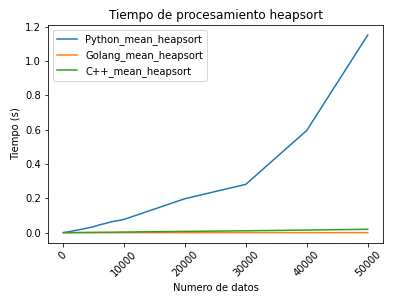
\includegraphics[width=0.8\textwidth]{Imagen/GHS1.png}
\label{fig:QuickSort}
\end{figure}

\begin{figure}[H]
\centering
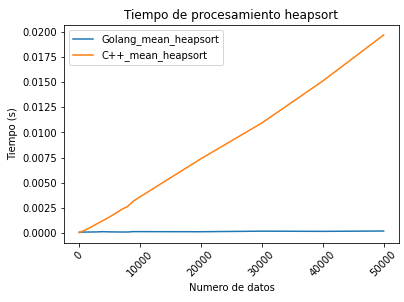
\includegraphics[width=0.8\textwidth]{Imagen/GHS2.png}
\label{fig:QuickSort}
\end{figure}

\begin{figure}[H]
\centering
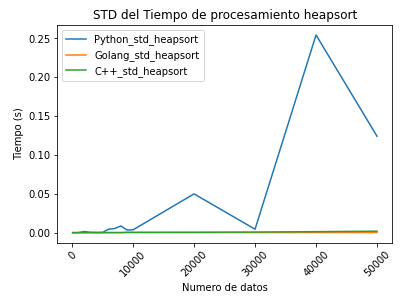
\includegraphics[width=0.8\textwidth]{Imagen/GHS3.png}
\label{fig:QuickSort}
\end{figure}

\begin{figure}[H]
\centering
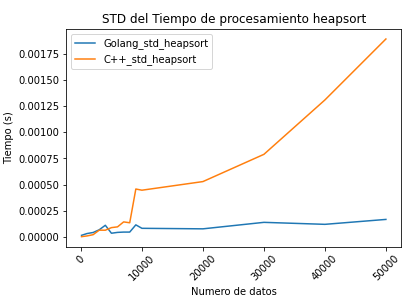
\includegraphics[width=0.8\textwidth]{Imagen/GHS4.png}
\label{fig:QuickSort}
\end{figure}

        \item Algoritmo Quick Sort
        
\begin{tabular}{ |p{0.3cm}||p{0.9cm}|p{1.5cm}|p{1.7cm}|p{1.5cm}|p{1.7cm}|p{1.8cm}|p{1.7cm}|  }
 \hline
 \multicolumn{8}{|c|}{Tabla comparativa con el promedio de tiempo de procesamiento y desviación estandar} \\
 \hline
 N°& Datos &Python Promedio &Python Desviación Estandar &C++ Promedio &C++ Desviación Estandar &GO Promedio &GO Desviación Estandar\\
 \hline
 1&100 &0.000134 &0.000007 &0.000018 &0.000008 &0.000071 &0.000015\\
 2&1000 &0.002729 &0.001485 &0.001017 &0.000452 &0.000067 &0.000006\\
 3&2000 &0.004458 &0.000247 &0.003921 &0.001844 &0.000072 &0.000020\\
 4&3000 &0.007151 &0.000272 &0.008771 &0.004201 &0.000088 &0.000033\\
 5&4000 &0.009444 &0.000111 &0.015590 &0.007550 &0.000076 &0.000028\\
 6&5000 &0.012021 &0.000038 &0.024317 &0.011846 &0.000078 &0.000048\\
 7&6000 &0.015133 &0.000416 &0.034986 &0.017096 &0.000075 &0.000027\\
 8&7000 &0.020725 &0.002518 &0.047467 &0.023276 &0.000070 &0.000015\\
 9&8000 &0.034460 &0.007882 &0.062724 &0.030843 &0.000069 &0.000007\\
 10&9000 &0.048326 &0.003676 &0.079264 &0.039038 &0.000079 &0.000056\\
 11&10000 &0.056400 &0.006677 &0.098758 &0.048722 &0.000074 &0.000030\\
 12&20000 &0.153343 &0.038574 &0.390520 &0.193812 &0.000075 &0.000026\\
 13&30000 &0.093278 &0.003922 &0.881592 &0.438707 &0.000110 &0.000053\\
 14&40000 &0.129151 &0.006084 &1.568770 &0.781403 &0.000089 &0.000030\\
 15&50000 &0.164665 &0.006518 &2.435630 &1.213870 &0.000093 &0.000044\\
 \hline
\end{tabular}

\begin{figure}[H]
\centering
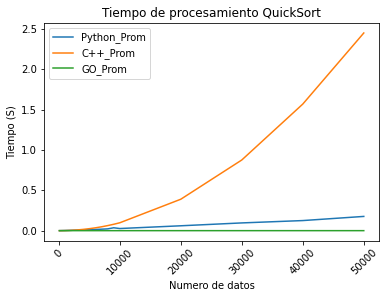
\includegraphics[width=0.8\textwidth]{Imagen/TP_QuickSort.png}
\caption{Tiempo de Procesamiento QuickSort}
\label{fig:QuickSort}
\end{figure}

\begin{figure}[H]
\centering
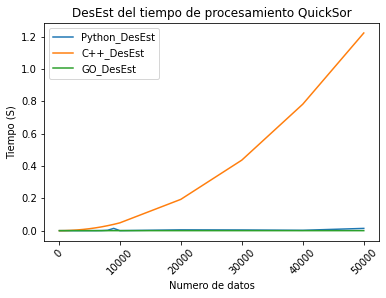
\includegraphics[width=0.8\textwidth]{Imagen/DE_QuickSort.png}
\caption{Desviación Estandar QuickSort}
\label{fig:QuickSort}
\end{figure}
  
        
        
        
    \end{enumerate}

\section{Conclusiones}

\begin{itemize}
            \item Para el Ordenamiento Rápido (QuickSort), se obtiene que el Tiempo de Procesamiento es menor en el lenguaje Goland, y el costo más alto es el lenguaje C++. Y la Desviación Estandar es similar entre los lenguajes de programación Python y Goland mientras que es mucho más alto en el lenguaje C++, lo que quiere decir que la dispersión de datos es mayor en esta última.
\end{itemize}
\begin{itemize}
            \item Para Counting Sort, se obtiene que el Tiempo de Procesamiento es menor en Goland, el costo más alto en Python y la Desviación Estandar es similar entre los lenguajes de programación C++ y Goland mientras que es mucho más alto en Python, lo que quiere decir que la dispersión de datos es mayor en esta última.
\end{itemize}

\begin{itemize}
            \item Para Merge Sort se obtiene que el Tiempo de Procesamiento es menor en Goland, incluso menor a C++, esto debido a que los programas en Go aprovechan mas fácil el paralelismo disponible, el tiempo fue mayor con Python. En cuanto a la Desviación Estandar la dispersión es mayor en Python y mucho menor en C++ y Goland.
\end{itemize}    
\begin{itemize}
            \item Cada lenguaje hace optimizaciones diferentes por lo que no tardan lo mismo, es decir cuando codificas en Python o Golang usando sus respectivas librerias realmente aprovechamos las optimizaciones que tienen en sus algoritmos internos para cada funcion, que pueden llamarse de la misma manera pero la implementacion optimiza algo del procesador.
\end{itemize}
\begin{itemize}
            \item C++ es el mas rapido en ejecutar codigo de maquina, pero el algoritmo puede hacer que incluso en el caso de Python o Golan ejecutando mas instrucciones, el total de intrucciones ejecutadas para procesar todo el conjunto de datos sea menor, aparentando ser mas rapido cuando solo es mas eficiente, que es lo que sucedio en Golang nos dio menores tiempos al procesar los ordenamientos.
\end{itemize}	
	%\clearpage
	%\bibliographystyle{apalike}
	%\bibliographystyle{IEEEtranN}
	%\bibliography{bibliography}
		
	
\end{document}

